\documentclass[12pt]{article}

\usepackage{amssymb,amsmath}
\usepackage[margin=1.0in]{geometry}
\usepackage{fancyhdr} % required for custom header
\usepackage{graphicx}
\usepackage{listings}
\usepackage{courier}
\usepackage{natbib}
\usepackage[usenames,dvipsnames]{color}

%set up the header
\pagestyle{fancy}
\lhead{Trever T. Hines}
\chead{RO 16-15 Reasearch Proposal}
\rhead{\today}

\setlength{\headheight}{15pt}
\renewcommand\headrulewidth{1.0pt} % Size of the header rule

%% Title
%%------------------------------------------------------------------------------
\title{	
 \rule{\headwidth}{1.0pt}
 Research proposal for RO 16-15:
 Novel crustal deformation models \
 characterizing earthquake hazard and its uncertainties in the western U.S.\
 \rule{\headwidth}{1.0pt}
 \author{Trever T. Hines}}

\begin{document}
\maketitle

\section*{Research Objective}
An accurate assessment of seismic hazard requires estimates of where faults have previously ruptured as well as the uncertainties on those estimates.  The research proposed here aims to address the latter. Finite fault rupture models, which are obtained through a regularized least squares inversion of geodetic data, lack meaningful quantifications of uncertainty. This is because model uncertainties are highly dependent upon the choice of regularization, which is subjective.  Although adding regularization to rupture models can result in a dubious solution, it is a necessity because an unregularized  solution may predict magnitudes and directions of fault slip that are clearly not physically plausible.  While the motivation behind regularization is to obtain a physically plausible model, the regularization schemes which are often employed, such as imposing smallness or smoothness on the solution, are not based on any empirical or theoretical studies.  The task is then to find a means of regularizing finite fault rupture models which is justified by our understanding how faults rupture.  In such case, regularization can be viewed as adding a prior constraint in a Bayesian sense, and the posterior ensemble of rupture models would provide a meaningful quantification of uncertainty.

We consider three well established, empirically derived relationships to use as prior constraints for rupture models. (1) Faults slip in the direction of maximum shear stress, $\sigma_\parallel$, \citep{Wallace1951}; (2) slip occurs when the Mohr-Coulomb failure criterion is exceeded \citep{Byerlee1978}; and (3) shear stress drop, $\Delta \sigma_\parallel$, tends to be in the range of 0.1 to 10 MPa, regardless of the spatial extent and magnitude of the earthquake \citep{Kanamori1975,Shearer2006}.  Constructing a prior based on the first two relationships would require an understanding of the ambient pre-seismic stress.  To constrain the direction on fault slip, only the orientation of the ambient stress needs to be known, which can be estimated from background seismicity.  The absolute ambient stress is necessary if we want to form a prior from the Mohr-Coulomb failure criterion, which states that
\begin{equation}\label{eq:MohrCoulomb}
  \mathbf{\sigma_\parallel} = C + \mu \mathbf{\sigma_\bot},
\end{equation}
where $\sigma_\bot$ is the normal stress on a fault, $C$ is cohesion, and $\mu$ is the coefficient of friction.  Barring earthquakes that produce significant stress overshoot, we can argue that the shear stress drop at any point on a fault cannot exceed its frictional strength.  Additionally, the coseismic increase in shear stress along the edges of a rupture zone cannot exceed the frictional strength. In order to calculate the maximum shear stress on a fault, we can assume that the normal stress on a strike-slip fault is primarily due to overburden.  Indirect inferences of the San Andreas fault strength which are based on heat flow and stress orientations across the fault find that $\mu\approx0.1$ \citep{Brune1969,Zoback1987}.  Laboratory experiments on gouge taken from the San Andreas fault find $\mu\approx0.3$ \citep{Carpenter2011}, while even higher values of 0.6 to 1.0 are suggested by \citet{Byerlee1978}. Even though the coefficient of friction can be debatable, we only need a reasonable upper bound on $\mu$ in order to limit the maximum shear stress drop in a rupture model.  Assuming no cohesion and $\mu\approx0.3$ \citep{Carpenter2011}, we can estimate that the shear stress required for an earthquake is on the order of 100 MPa and thus $|\Delta\sigma_\parallel|\lesssim 100 $ MPa everywhere on the fault.  This can then be used to constrain $\Delta u$ through the relationship
\begin{equation}\label{eq:StressSlip}
  \Delta \sigma_\parallel (\xi_1) = \int_F K(\xi_1,\xi_2) \Delta u(\xi_2) d\xi_2,
\end{equation}
where $K(\xi_1,\xi_2)$ describes the stress drop at $\xi_1$ resulting from slip at $\xi_2$, and $F$ denotes the fault.  When assuming that our domain is a homogeneous, isotropic, elastic, half-space, we can compute $K$ with the analytical solution from \citet{Okada1992}.  

The observation that stress drop is consistently on the order of 0.1 to 10 MPa offers a tighter constraint on fault slip than the Mohr-Coulomb failure criterion.  Seismologically determined stress drops can be interpreted as the average coseismic change in shear stress over the rupture zone.  The difficulty is that we do not know the rupture zone \textit{a priori}, since that is what we are trying to estimate in a finite fault rupture model.  However, we do know that stress drop is invariant to the spatial extent of the earthquake and thus we can posit that the stress drop at each point on a ruptured fault should also be subject to the same bounds of 0.1 to 10 MPa.  Outside of the rupture zone, stress drop will generally be negative (i.e. pushed closer to failure).  When considering the entire fault, not just the area that ruptured, we can then impose an upper bound of 10 MPa on $\Delta \sigma_\parallel$.  

We use a synthetic test to demonstrate how effectively these physical constraints regularize finite fault rupture models.  A thoroughly annotated IPython notebook containing all the work done for this synthetic test can be found in www.github.com/treverhines/ MendenhallProposal.git.  In this synthetic test, we invert displacements resulting from slip on an infinitely long, strike-slip fault embedded in a homogeneous, elastic half-space.  This problem degenerates to a two-dimensional problem where the fault strike and displacements are in the anti-plane direction.  The fault extends from the surface to 15 km depth and is discretized into 10 segments.  We impose slip which is consistent with a uniform stress drop of 5 MPa.  The slip and resulting displacements, with added noise, are shown in Figure 1.

Inverting surface displacements for fault slip is typically done by using regularized least squares to solve
\begin{equation}\label{eq:Forward}
  u(x) = \int_F G(x,\xi) \Delta u(\xi) d\xi,
\end{equation}
where $u(x)$ are the observable coseismic surface displacements, and $G(x,\xi)$ describes displacements at $x$ resulting from slip at $\xi$.  For this two-dimensional problem the maximum shear stress direction is in the anti-plane direction and we can enforce $\Delta u$ to be in the same direction by solving eq. \ref{eq:Forward} with a bounded least squares algorithm \citep{Lawson1995}.  If we wished to solve eq. \ref{eq:Forward} with constraints on $\Delta \sigma_\parallel$ rather than $\Delta u$, then the inverse of eq. \ref{eq:StressSlip} can be combined with eq. \ref{eq:Forward}, and then that equation can be solved with bounded least squares. We wish to put constraints on both $\Delta u$ and $\Delta \sigma_\parallel$, and there is not immediately apparent way to impose such constraints with bounded least squares.  We then resort to the more expensive, although more informative, Monte Carlo methods.  Specifically, we use a Metropolis-Hastings algorithm to estimate $\Delta u$ with the prior constraint that $\Delta u$ is positive and $\Delta \sigma_\parallel < 10$ MPa for each fault segment.  We also add a prior constraint on the seismic potency, which we define for this two-dimensional problem as the average slip multiplied by the fault width.  The seismic potency for the true model is 0.58 $\mathrm{km}^2$ and we use a prior with a mean of  0.6 $\mathrm{km}^2$ and standard deviation of 0.1 $\mathrm{km}^2$.  

For each iteration in the Metropolis-Hastings algorithm, the likelihood of a trial model is calculated based on how well it agrees with our prior and how well it agrees with the observed data.  If we have $N$ observations and $M$ unknown model parameters, then the computational cost of comparing the predictions of the trial model to the observed data is $O(NM)$. The cost of testing if a trial model agrees with our prior is $O(M^2)$, where the main burden is in evaluating eq. \ref{eq:StressSlip}.  However, the discretized matrix representing $K$ is sparse because stress drop on a fault segment is mostly a function of slip on nearby fault segments.  If we take advantage of this sparsity then the cost of comparing a test model to the prior is $O(M)$.  Thus, the main bottleneck in our algorithm is in comparing the observations to the predictions for each trial model. 

\begin{figure}
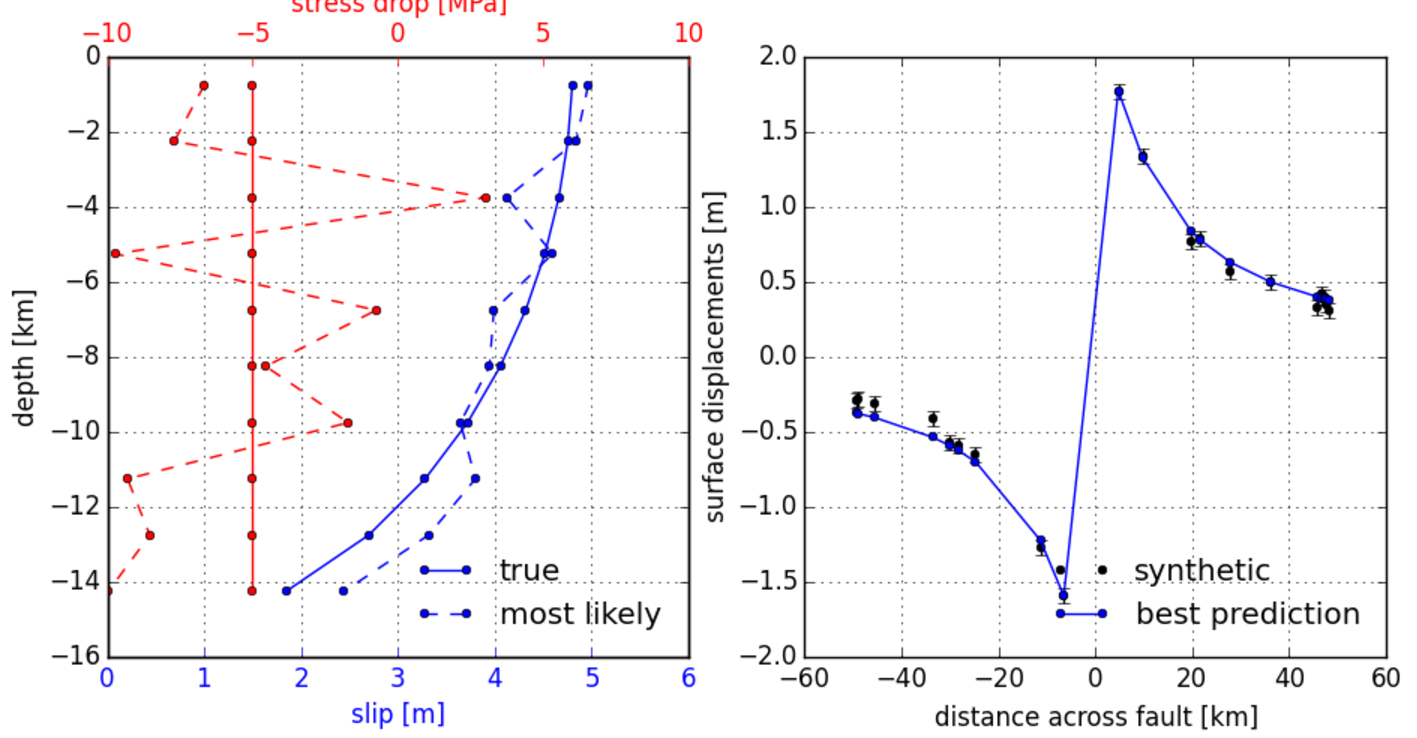
\includegraphics[width=1.0\textwidth]{figure_1}
\caption{Left: solid blue and red lines indicates the true slip and stress drop respectively, and dashed lines indicate the inferred slip and stress drop for the most likely posterior model.  Right: synthetic data with their 68\% confidence intervals are shown as black points, and the blue line is the prediction from the most likely posterior model.}  
\end{figure}

We ran one million iterations of the Metropolis-Hastings algorithm, which takes about one minute on a desktop computer.  Our most likely slip model is shown in Figure 1 along with the predicted displacements.  The posterior distribution of slip is shown in the left panel of Figure 2.  For comparison we ran another inversion without bounds on stress drop, and the posterior distribution is shown in the right panel in Figure 2.  When stress drop is unbounded, most of the retained models have no slip on all but a few fault segments, which then have 10s of meters of slip in order to produce the required potency.  As a result, the posterior slip distributions tend to be wide and have low mean values.  This is in sharp contrast to the posterior slip distribution when stress drop is bounded.  In this case, the posterior has mean values that closely match the true slip model. Perhaps surprisingly, slip is better resolved at greater depths. This is because the bounds on stress drop force the slip to taper to zero at or above 15 km depth.  


\begin{figure}
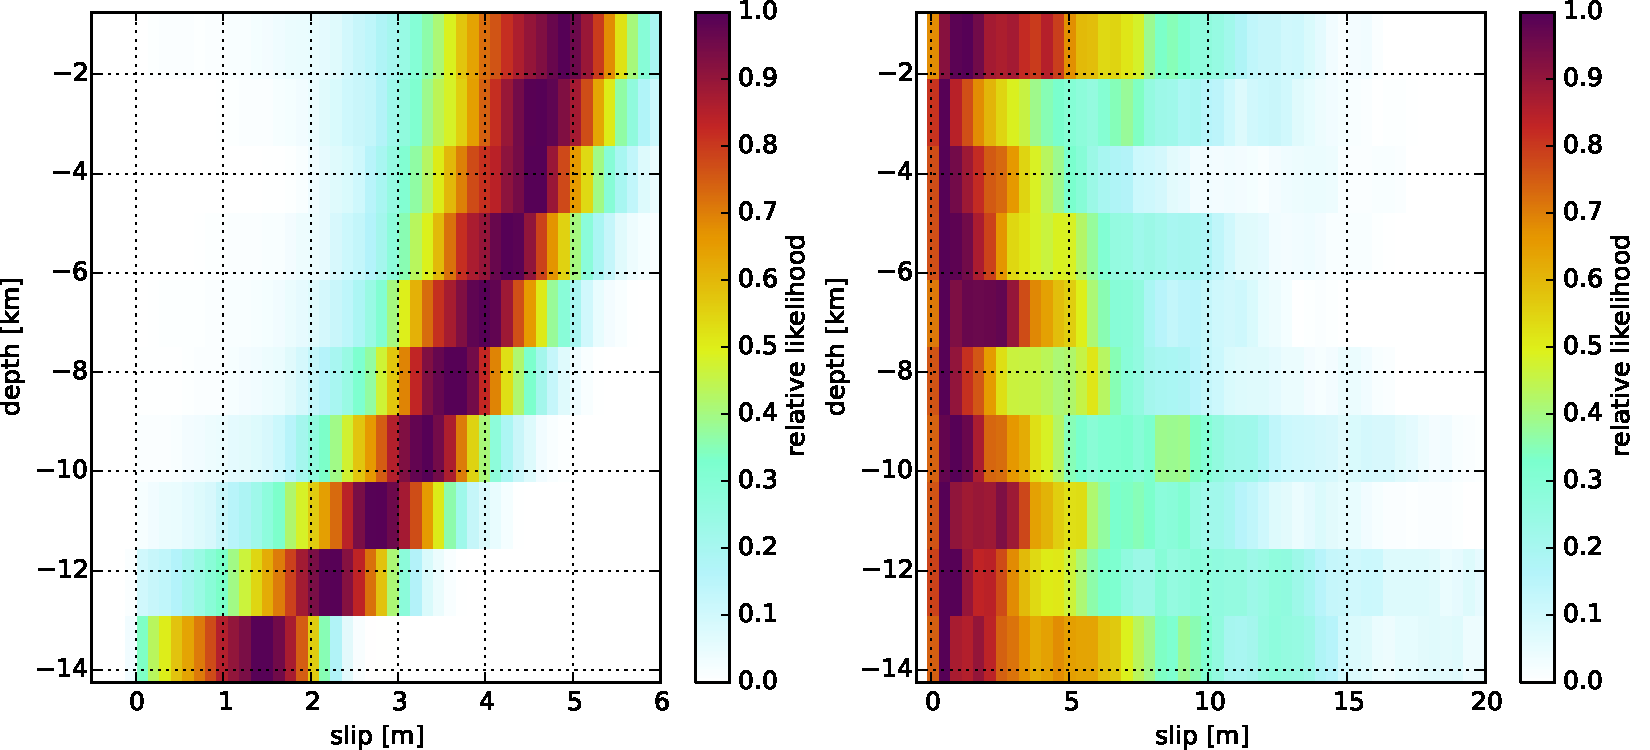
\includegraphics[width=1.0\textwidth]{figure_2}
\raggedleft
\caption{Left: marginal posterior probability density function of slip for each depth interval when stress drop is bounded to be less than 10 MPa (left) and when stress is unbounded (right).}  
\end{figure}

%\bibliography{mybib}{}
%\bibliographystyle{plain}
\bibliographystyle{apalike}
\bibliography{mybib}

\end{document}